% Compile with: pdflatex presentation.tex
\documentclass[aspectratio=169,10pt]{beamer}

% ============================================
% THEME & BASIC CONFIGURATION
% ============================================
\usetheme{default}
\setbeamertemplate{navigation symbols}{}
\setbeamertemplate{itemize items}[circle]
\setbeamertemplate{enumerate items}[default]

% ============================================
% COLOR PALETTE
% ============================================
\definecolor{primaryblue}{RGB}{41,65,114}
\definecolor{accentteal}{RGB}{72,149,159}
\definecolor{softcream}{RGB}{253,251,247}
\definecolor{warmpeach}{RGB}{255,218,193}
\definecolor{mintgreen}{RGB}{200,230,220}
\definecolor{softgray}{RGB}{245,245,248}
\definecolor{darktext}{RGB}{50,50,60}

\setbeamercolor{normal text}{fg=darktext}
\setbeamercolor{frametitle}{fg=primaryblue}
\setbeamercolor{itemize item}{fg=accentteal}
\setbeamercolor{enumerate item}{fg=primaryblue}

% ============================================
% PACKAGES
% ============================================
\usepackage{amsmath,amssymb}
\usepackage{booktabs}
\usepackage{tikz}
\usepackage{graphicx}
\usepackage[table]{xcolor}
\usetikzlibrary{shapes,arrows,positioning,calc,fit,backgrounds,shadows.blur}

% Custom frame title - compact
\setbeamertemplate{frametitle}{
    \vspace{0.15cm}
    {\large\bfseries\color{primaryblue}\insertframetitle}
    
\begin{tikzpicture}
        \fill[accentteal] (0,0) rectangle (1.8cm,1.5pt);
        \fill[warmpeach] (1.9cm,0) rectangle (2.3cm,1.5pt);
    \end{tikzpicture}
    \vspace{0cm}
}

% ============================================
% TITLE INFORMATION
% ============================================
\title{AetherScan}
\subtitle{Environmental Intelligence Platform for Real-Time Air Quality Monitoring}
\author{Pranjal Sailwal \and Prakriti Kimothi \and Sriya Rawat \and Siddhant Dabral}
\institute{Graphic Era Hill University, Dehradun}
\date{January 2026}

\begin{document}

% ============================================
% SLIDE 1: TITLE
% ============================================
\begin{frame}[plain]
\begin{tikzpicture}[remember picture,overlay]
    \fill[softcream] (current page.south west) rectangle (current page.north east);
    % Top decoration
    \fill[primaryblue!15] ([xshift=-1cm]current page.north west)
        .. controls +(3,-0.5) and +(-2,2) .. ([xshift=4cm,yshift=-1.5cm]current page.north west)
        -- ([xshift=-1cm,yshift=-1.5cm]current page.north west) -- cycle;
    \fill[warmpeach!50] ([xshift=2cm,yshift=-0.8cm]current page.north west) circle (0.25cm);
    % Bottom decoration
    \fill[accentteal!12] ([xshift=1cm]current page.south east)
        .. controls +(-3,0.5) and +(2,-2) .. ([xshift=-4cm,yshift=1.5cm]current page.south east)
        -- ([xshift=1cm,yshift=1.5cm]current page.south east) -- cycle;
    \fill[mintgreen!60] ([xshift=-2.5cm,yshift=1.2cm]current page.south east) circle (0.2cm);
\end{tikzpicture}

\vspace{0.8cm}
\begin{center}
    {\fontsize{36}{42}\selectfont\bfseries\color{primaryblue} AetherScan}
    \vspace{0.3cm}

    
\begin{tikzpicture}
        \fill[accentteal] (-1.5,0) rectangle (1.5,1.5pt);
    \end{tikzpicture}
    \vspace{0.2cm}

    {\normalsize\color{darktext} Environmental Intelligence Platform for\\[0.15cm] Real-Time Air Quality Monitoring}
    \vspace{0.6cm}

    
\begin{tikzpicture}
        \node[rounded corners=6pt, fill=white, drop shadow={opacity=0.15}, inner sep=10pt] {
            \small
            \textbf{\color{primaryblue}Pranjal Sailwal} \quad
            \textbf{\color{primaryblue}Prakriti Kimothi} \quad
            \textbf{\color{primaryblue}Sriya Rawat} \quad
            \textbf{\color{primaryblue}Siddhant Dabral}
        };
    \end{tikzpicture}
    \vspace{0.4cm}

    {\footnotesize\color{darktext!80} Department of Computer Science and Engineering\\
    Graphic Era Hill University, Dehradun}
    \vspace{0.2cm}

    {\footnotesize\color{accentteal}\textbf{Mentor:} Dr. Susheela Dahiya}
\end{center}
\end{frame}

% ============================================
% SLIDE 2: PROBLEM CONTEXT
% ============================================
\begin{frame}{Problem Context}
\begin{columns}[T]
    \begin{column}{0.52\textwidth}
        \textbf{\color{primaryblue}Air Quality Challenges in India}
        \vspace{0.15cm}

        \small
        \begin{itemize}\setlength{\itemsep}{3pt}
            \item Multiple Indian cities rank among world's most polluted urban centers
            \item Monitoring data scattered across different government and international platforms
            \item Sparse sensor coverage leaves significant geographic gaps in rural areas
            \item Technical complexity prevents general public from accessing actionable insights
        \end{itemize}

        \vspace{0.25cm}
        \textbf{\color{primaryblue}Identified Research Gap}
        \vspace{0.1cm}

        \begin{itemize}\setlength{\itemsep}{3pt}
            \item No unified platform integrating multiple authoritative data sources
            \item Limited spatial interpolation methods for continuous coverage
            \item Absence of comprehensive analytical and reporting tools
        \end{itemize}
    \end{column}

    \begin{column}{0.45\textwidth}
        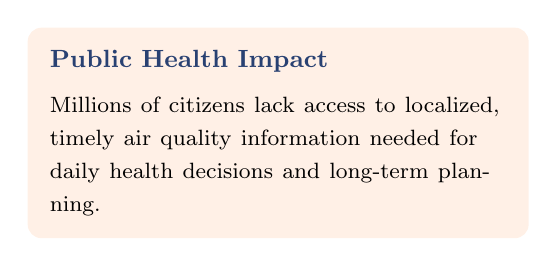
\begin{tikzpicture}
            \node[rounded corners=5pt, fill=warmpeach!40, inner sep=8pt, text width=5.8cm] {
                \textbf{\color{primaryblue}\small Public Health Impact}\\[0.15cm]
                \footnotesize Millions of citizens lack access to localized, timely air quality information needed for daily health decisions and long-term planning.
            };
        \end{tikzpicture}

        \vspace{0.25cm}

        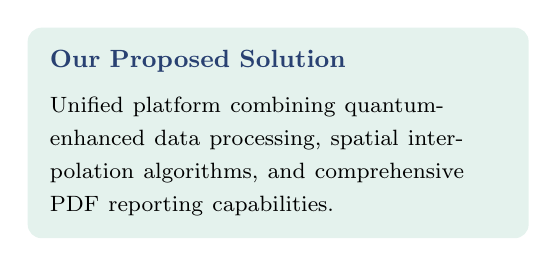
\begin{tikzpicture}
            \node[rounded corners=5pt, fill=mintgreen!50, inner sep=8pt, text width=5.8cm] {
                \textbf{\color{primaryblue}\small Our Proposed Solution}\\[0.15cm]
                \footnotesize Unified platform combining quantum-enhanced data processing, spatial interpolation algorithms, and comprehensive PDF reporting capabilities.
            };
        \end{tikzpicture}

        \vspace{0.25cm}

        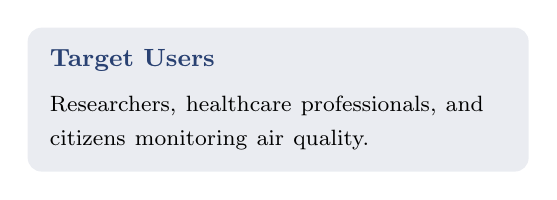
\begin{tikzpicture}
            \node[rounded corners=5pt, fill=primaryblue!10, inner sep=8pt, text width=5.8cm] {
                \textbf{\color{primaryblue}\small Target Users}\\[0.15cm]
                \footnotesize Researchers, healthcare professionals, and citizens monitoring air quality.
            };
        \end{tikzpicture}
    \end{column}
\end{columns}
\end{frame}

% ============================================
% SLIDE 3: OBJECTIVES
% ============================================
\begin{frame}{Project Objectives}
\begin{columns}[T]
    \begin{column}{0.48\textwidth}
        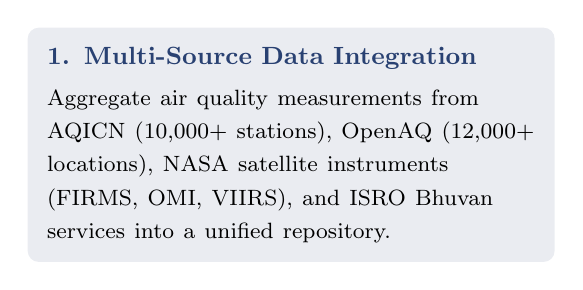
\begin{tikzpicture}
            \node[rounded corners=4pt, fill=primaryblue!10, inner sep=7pt, text width=6.2cm] {
                \textbf{\color{primaryblue}\small 1. Multi-Source Data Integration}\\[0.1cm]
                \footnotesize Aggregate air quality measurements from AQICN (10,000+ stations), OpenAQ (12,000+ locations), NASA satellite instruments (FIRMS, OMI, VIIRS), and ISRO Bhuvan services into a unified repository.
            };
        \end{tikzpicture}

        \vspace{0.15cm}

        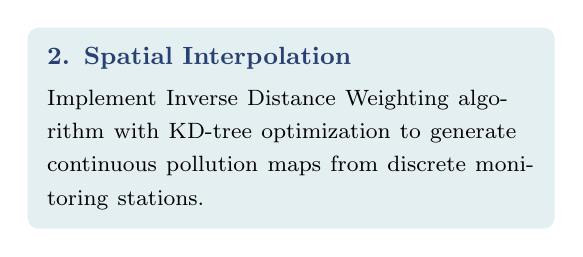
\begin{tikzpicture}
            \node[rounded corners=4pt, fill=accentteal!15, inner sep=7pt, text width=6.2cm] {
                \textbf{\color{primaryblue}\small 2. Spatial Interpolation}\\[0.1cm]
                \footnotesize Implement Inverse Distance Weighting algorithm with KD-tree optimization to generate continuous pollution maps from discrete monitoring stations.
            };
        \end{tikzpicture}

        \vspace{0.15cm}

        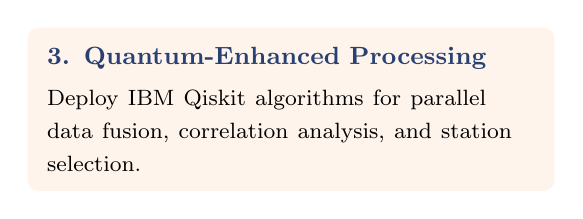
\begin{tikzpicture}
            \node[rounded corners=4pt, fill=warmpeach!30, inner sep=7pt, text width=6.2cm] {
                \textbf{\color{primaryblue}\small 3. Quantum-Enhanced Processing}\\[0.1cm]
                \footnotesize Deploy IBM Qiskit algorithms for parallel data fusion, correlation analysis, and station selection.
            };
        \end{tikzpicture}
    \end{column}

    \begin{column}{0.48\textwidth}
        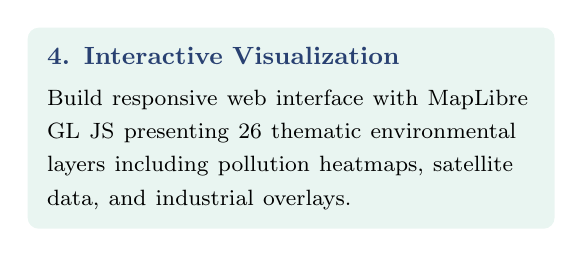
\begin{tikzpicture}
            \node[rounded corners=4pt, fill=mintgreen!40, inner sep=7pt, text width=6.2cm] {
                \textbf{\color{primaryblue}\small 4. Interactive Visualization}\\[0.1cm]
                \footnotesize Build responsive web interface with MapLibre GL JS presenting 26 thematic environmental layers including pollution heatmaps, satellite data, and industrial overlays.
            };
        \end{tikzpicture}

        \vspace{0.15cm}

        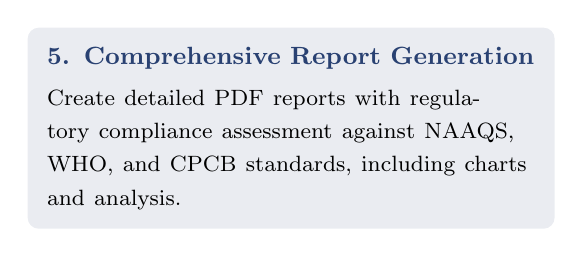
\begin{tikzpicture}
            \node[rounded corners=4pt, fill=primaryblue!10, inner sep=7pt, text width=6.2cm] {
                \textbf{\color{primaryblue}\small 5. Comprehensive Report Generation}\\[0.1cm]
                \footnotesize Create detailed PDF reports with regulatory compliance assessment against NAAQS, WHO, and CPCB standards, including charts and analysis.
            };
        \end{tikzpicture}

        \vspace{0.15cm}

        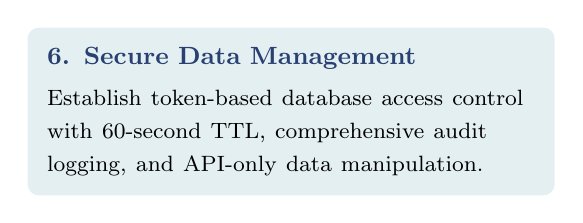
\begin{tikzpicture}
            \node[rounded corners=4pt, fill=accentteal!15, inner sep=7pt, text width=6.2cm] {
                \textbf{\color{primaryblue}\small 6. Secure Data Management}\\[0.1cm]
                \footnotesize Establish token-based database access control with 60-second TTL, comprehensive audit logging, and API-only data manipulation.
            };
        \end{tikzpicture}
    \end{column}
\end{columns}
\end{frame}

% ============================================
% SLIDE 4: SYSTEM ARCHITECTURE
% ============================================
\begin{frame}{System Architecture}
\begin{columns}[T]
    \begin{column}{0.55\textwidth}
        \begin{center}
        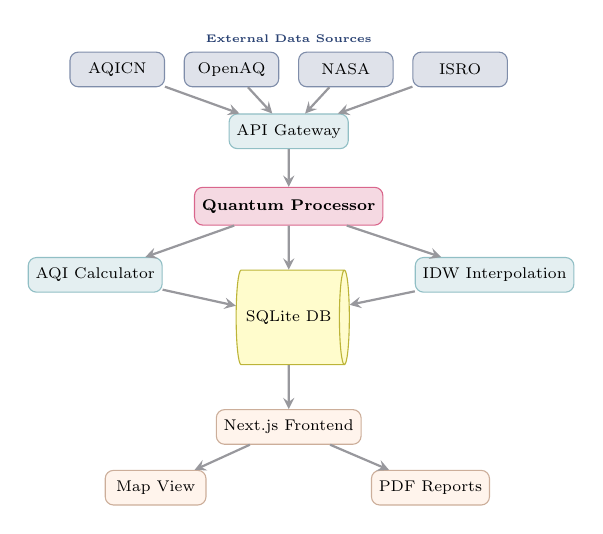
\begin{tikzpicture}[
            scale=0.8,
            transform shape,
            node distance=0.6cm,
            every node/.style={font=\scriptsize},
            datasource/.style={rectangle, rounded corners=3pt, draw=primaryblue!60, fill=primaryblue!15,
                               minimum width=1.5cm, minimum height=0.55cm},
            process/.style={rectangle, rounded corners=3pt, draw=accentteal!60, fill=accentteal!15,
                            minimum width=1.8cm, minimum height=0.55cm},
            quantum/.style={rectangle, rounded corners=3pt, draw=purple!60, fill=purple!15,
                            minimum width=2.2cm, minimum height=0.6cm, font=\scriptsize\bfseries},
            storage/.style={cylinder, draw=yellow!70!black, fill=yellow!20,
                            minimum width=1.5cm, minimum height=0.45cm, aspect=0.35},
            frontend/.style={rectangle, rounded corners=3pt, draw=warmpeach!80!black, fill=warmpeach!30,
                             minimum width=1.6cm, minimum height=0.55cm},
            arrow/.style={->,>=stealth,thick,color=darktext!50}
        ]

        \node[datasource] (aqicn) {AQICN};
        \node[datasource, right=0.3cm of aqicn] (openaq) {OpenAQ};
        \node[datasource, right=0.3cm of openaq] (nasa) {NASA};
        \node[datasource, right=0.3cm of nasa] (isro) {ISRO};

        \node[above=0.3cm of $(openaq)!0.5!(nasa)$, font=\tiny\color{primaryblue}] {\textbf{External Data Sources}};

        \node[process, below=0.7cm of $(openaq)!0.5!(nasa)$] (api) {API Gateway};
        \node[quantum, below=0.6cm of api] (quantum) {Quantum Processor};
        \node[process, below left=0.5cm and 0.5cm of quantum] (aqi) {AQI Calculator};
        \node[process, below right=0.5cm and 0.5cm of quantum] (idw) {IDW Interpolation};
        \node[storage, below=0.7cm of quantum] (db) {SQLite DB};
        \node[frontend, below=0.7cm of db] (front) {Next.js Frontend};
        \node[frontend, below left=0.4cm and 0.15cm of front] (map) {Map View};
        \node[frontend, below right=0.4cm and 0.15cm of front] (pdf) {PDF Reports};

        \draw[arrow] (aqicn) -- (api);
        \draw[arrow] (openaq) -- (api);
        \draw[arrow] (nasa) -- (api);
        \draw[arrow] (isro) -- (api);
        \draw[arrow] (api) -- (quantum);
        \draw[arrow] (quantum) -- (aqi);
        \draw[arrow] (quantum) -- (idw);
        \draw[arrow] (quantum) -- (db);
        \draw[arrow] (aqi) -- (db);
        \draw[arrow] (idw) -- (db);
        \draw[arrow] (db) -- (front);
        \draw[arrow] (front) -- (map);
        \draw[arrow] (front) -- (pdf);

        \end{tikzpicture}
        \end{center}
    \end{column}

    \begin{column}{0.43\textwidth}
        \textbf{\color{primaryblue}\small Architecture Highlights}
        \vspace{0.15cm}

        \footnotesize
        \begin{itemize}\setlength{\itemsep}{4pt}
            \item \textbf{Data Layer:} Eight external APIs 
            \item \textbf{Processing Layer:} Quantum processor handles all data fusion before storage
            \item \textbf{Storage Layer:} SQLite with token-based security middleware
            \item \textbf{Presentation Layer:} React/Next.js frontend with MapLibre GL
        \end{itemize}

        \vspace{0.2cm}

        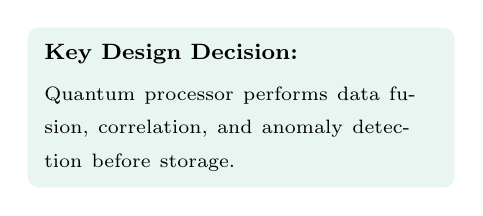
\begin{tikzpicture}
            \node[rounded corners=4pt, fill=mintgreen!40, inner sep=6pt, text width=5cm] {
                \footnotesize\textbf{Key Design Decision:}\\[0.1cm]
                \scriptsize Quantum processor performs data fusion, correlation, and anomaly detection before storage.
            };
        \end{tikzpicture}

        \vspace{0.15cm}

        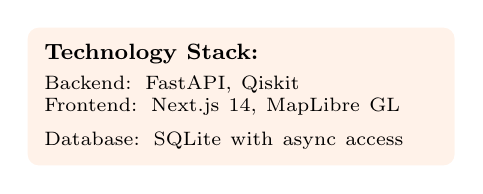
\begin{tikzpicture}
            \node[rounded corners=4pt, fill=warmpeach!35, inner sep=6pt, text width=5cm] {
                \footnotesize\textbf{Technology Stack:}\\[0.1cm]
                \scriptsize Backend: FastAPI, Qiskit\\
                Frontend: Next.js 14, MapLibre GL\\
                Database: SQLite with async access
            };
        \end{tikzpicture}
    \end{column}
\end{columns}
\end{frame}

% ============================================
% SLIDE 5: AQI CALCULATION
% ============================================
\begin{frame}{Methodology: Air Quality Index Calculation}
\begin{columns}[T]
    \begin{column}{0.48\textwidth}
        \textbf{\color{primaryblue}\small CPCB Standard Method}
        \vspace{0.1cm}

        \footnotesize
        Six criteria pollutants: PM$_{2.5}$, PM$_{10}$, NO$_2$, SO$_2$, CO, O$_3$

        \vspace{0.15cm}
        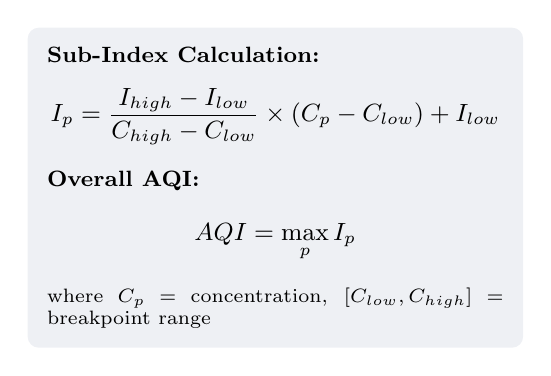
\begin{tikzpicture}
            \node[rounded corners=4pt, fill=primaryblue!8, inner sep=7pt] {
                \begin{minipage}{5.8cm}
                    \footnotesize\textbf{Sub-Index Calculation:}
                    \small
                    $$I_p = \frac{I_{high} - I_{low}}{C_{high} - C_{low}} \times (C_p - C_{low}) + I_{low}$$

                    \footnotesize\textbf{Overall AQI:}
                    \small
                    $$AQI = \max_{p} I_p$$

                    \scriptsize where $C_p$ = concentration, $[C_{low}, C_{high}]$ = breakpoint range
                \end{minipage}
            };
        \end{tikzpicture}

        \vspace{0.15cm}

        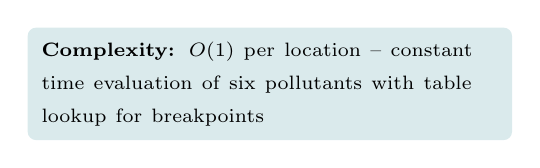
\begin{tikzpicture}
            \node[rounded corners=3pt, fill=accentteal!20, inner sep=5pt, text width=5.8cm] {
                \scriptsize\textbf{Complexity:} $O(1)$ per location -- constant time evaluation of six pollutants with table lookup for breakpoints
            };
        \end{tikzpicture}
    \end{column}

    \begin{column}{0.48\textwidth}
        \textbf{\color{primaryblue}\small AQI Category Breakpoints}
        \vspace{0.1cm}

        \scriptsize
        \renewcommand{\arraystretch}{1.05}
        \begin{tabular}{p{1.8cm}ccc}
            \rowcolor{green!20} Good & 0--50 & PM$_{2.5}$: 0--30 \\
            \rowcolor{yellow!20} Satisfactory & 51--100 & PM$_{2.5}$: 31--60 \\
            \rowcolor{orange!20} Moderate & 101--200 & PM$_{2.5}$: 61--90 \\
            \rowcolor{red!15} Poor & 201--300 & PM$_{2.5}$: 91--120 \\
            \rowcolor{purple!15} Very Poor & 301--400 & PM$_{2.5}$: 121--250 \\
            \rowcolor{red!30} Severe & 401--500 & PM$_{2.5}$: $>$250 \\
        \end{tabular}

        \vspace{0.2cm}

        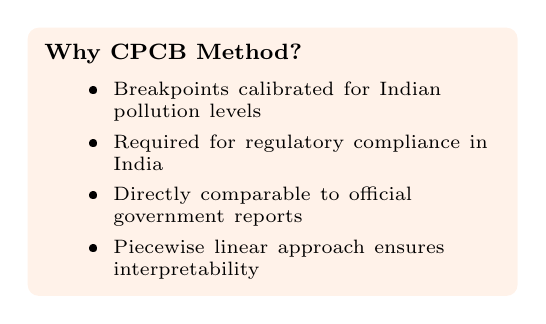
\begin{tikzpicture}
            \node[rounded corners=4pt, fill=warmpeach!35, inner sep=6pt, text width=5.8cm] {
                \footnotesize\textbf{Why CPCB Method?}\\[0.1cm]
                \scriptsize
                \begin{itemize}\setlength{\itemsep}{1pt}
                    \item Breakpoints calibrated for Indian pollution levels
                    \item Required for regulatory compliance in India
                    \item Directly comparable to official government reports
                    \item Piecewise linear approach ensures interpretability
                \end{itemize}
            };
        \end{tikzpicture}
    \end{column}
\end{columns}
\end{frame}

% ============================================
% SLIDE 6: IDW INTERPOLATION
% ============================================
\begin{frame}{Methodology: Inverse Distance Weighting Interpolation}
\begin{columns}[T]
    \begin{column}{0.50\textwidth}
        \textbf{\color{primaryblue}\small Purpose}
        \vspace{0.05cm}

        \footnotesize
        Generate continuous pollution maps from sparse monitoring stations

        \vspace{0.15cm}
        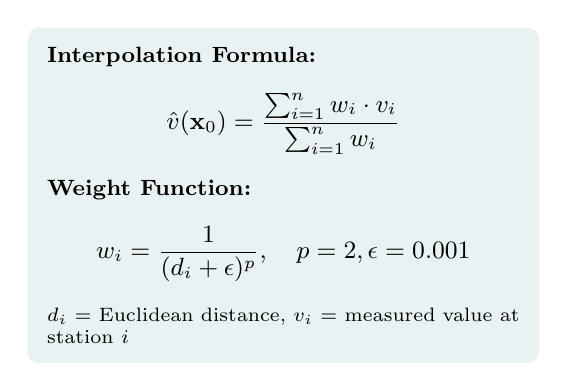
\begin{tikzpicture}
            \node[rounded corners=4pt, fill=accentteal!12, inner sep=7pt] {
                \begin{minipage}{6cm}
                    \footnotesize\textbf{Interpolation Formula:}
                    \small
                    $$\hat{v}(\mathbf{x}_0) = \frac{\sum_{i=1}^{n} w_i \cdot v_i}{\sum_{i=1}^{n} w_i}$$

                    \footnotesize\textbf{Weight Function:}
                    \small
                    $$w_i = \frac{1}{(d_i + \epsilon)^p}, \quad p = 2, \epsilon = 0.001$$

                    \scriptsize $d_i$ = Euclidean distance, $v_i$ = measured value at station $i$
                \end{minipage}
            };
        \end{tikzpicture}

        \vspace{0.15cm}
        \textbf{\color{primaryblue}\footnotesize KD-Tree Optimization}
        \scriptsize
        \begin{itemize}\setlength{\itemsep}{2pt}
            \item Tree construction: $O(n \log n)$
            \item Nearest neighbor query: $O(k \log n)$
            \item National grid (100k points): $<$3 seconds
        \end{itemize}
    \end{column}

    \begin{column}{0.47\textwidth}
        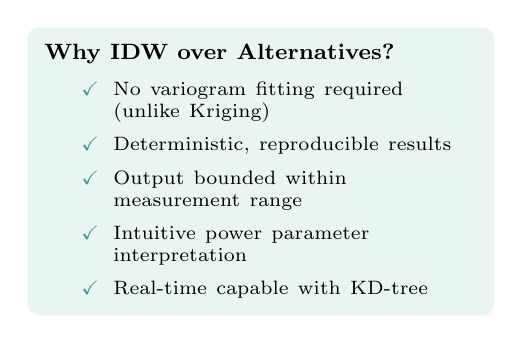
\begin{tikzpicture}
            \node[rounded corners=4pt, fill=mintgreen!40, inner sep=6pt, text width=5.5cm] {
                \footnotesize\textbf{Why IDW over Alternatives?}\\[0.1cm]
                \scriptsize
                \begin{itemize}\setlength{\itemsep}{2pt}
                    \item[\color{accentteal}$\checkmark$] No variogram fitting required (unlike Kriging)
                    \item[\color{accentteal}$\checkmark$] Deterministic, reproducible results
                    \item[\color{accentteal}$\checkmark$] Output bounded within measurement range
                    \item[\color{accentteal}$\checkmark$] Intuitive power parameter interpretation
                    \item[\color{accentteal}$\checkmark$] Real-time capable with KD-tree
                \end{itemize}
            };
        \end{tikzpicture}

        \vspace{0.15cm}

        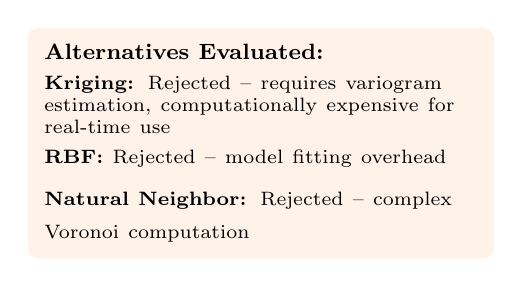
\begin{tikzpicture}
            \node[rounded corners=4pt, fill=warmpeach!35, inner sep=6pt, text width=5.5cm] {
                \footnotesize\textbf{Alternatives Evaluated:}\\[0.1cm]
                \scriptsize
                \textbf{Kriging:} Rejected -- requires variogram estimation, computationally expensive for real-time use\\[0.1cm]
                \textbf{RBF:} Rejected -- model fitting overhead\\[0.1cm]
                \textbf{Natural Neighbor:} Rejected -- complex Voronoi computation
            };
        \end{tikzpicture}

        \vspace{0.15cm}

        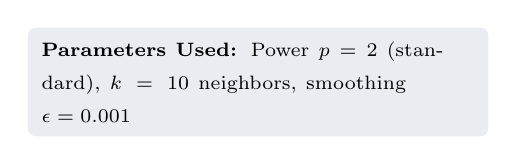
\begin{tikzpicture}
            \node[rounded corners=3pt, fill=primaryblue!10, inner sep=5pt, text width=5.5cm] {
                \scriptsize\textbf{Parameters Used:} Power $p=2$ (standard), $k=10$ neighbors, smoothing $\epsilon=0.001$
            };
        \end{tikzpicture}
    \end{column}
\end{columns}
\end{frame}

% ============================================
% SLIDE 7: QUANTUM SUPERPOSITION
% ============================================
\begin{frame}{Methodology: Quantum Superposition Processing}
\begin{columns}[T]
    \begin{column}{0.52\textwidth}
        \textbf{\color{primaryblue}\small Concept}
        \vspace{0.05cm}

        \footnotesize
        Process multiple data sources simultaneously using quantum superposition

        \vspace{0.15cm}
        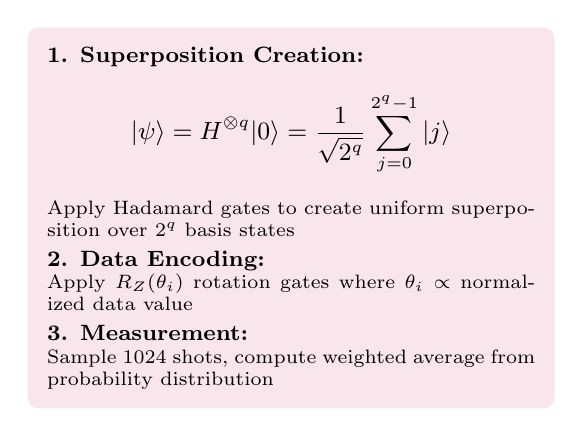
\begin{tikzpicture}
            \node[rounded corners=4pt, fill=purple!10, inner sep=7pt] {
                \begin{minipage}{6.2cm}
                    \footnotesize\textbf{1. Superposition Creation:}
                    \small
                    $$|\psi\rangle = H^{\otimes q}|0\rangle = \frac{1}{\sqrt{2^q}} \sum_{j=0}^{2^q-1} |j\rangle$$

                    \scriptsize Apply Hadamard gates to create uniform superposition over $2^q$ basis states

                    \vspace{0.1cm}
                    \footnotesize\textbf{2. Data Encoding:}\\
                    \scriptsize Apply $R_Z(\theta_i)$ rotation gates where $\theta_i \propto$ normalized data value

                    \vspace{0.1cm}
                    \footnotesize\textbf{3. Measurement:}\\
                    \scriptsize Sample 1024 shots, compute weighted average from probability distribution
                \end{minipage}
            };
        \end{tikzpicture}

        \vspace{0.1cm}
        
\begin{tikzpicture}
            \node[rounded corners=3pt, fill=accentteal!20, inner sep=4pt] {
                \scriptsize\textbf{Framework:} IBM Qiskit 0.45.1 Statevector Simulator
            };
        \end{tikzpicture}
    \end{column}

    \begin{column}{0.45\textwidth}
        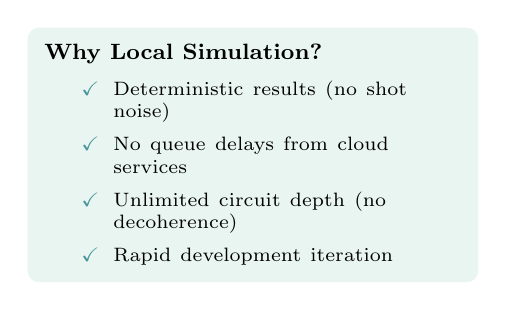
\begin{tikzpicture}
            \node[rounded corners=4pt, fill=mintgreen!40, inner sep=6pt, text width=5.3cm] {
                \footnotesize\textbf{Why Local Simulation?}\\[0.1cm]
                \scriptsize
                \begin{itemize}\setlength{\itemsep}{2pt}
                    \item[\color{accentteal}$\checkmark$] Deterministic results (no shot noise)
                    \item[\color{accentteal}$\checkmark$] No queue delays from cloud services
                    \item[\color{accentteal}$\checkmark$] Unlimited circuit depth (no decoherence)
                    \item[\color{accentteal}$\checkmark$] Rapid development iteration
                \end{itemize}
            };
        \end{tikzpicture}

        \vspace{0.15cm}

        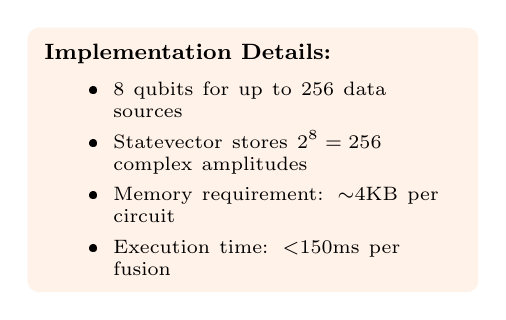
\begin{tikzpicture}
            \node[rounded corners=4pt, fill=warmpeach!35, inner sep=6pt, text width=5.3cm] {
                \footnotesize\textbf{Implementation Details:}\\[0.1cm]
                \scriptsize
                \begin{itemize}\setlength{\itemsep}{1pt}
                    \item 8 qubits for up to 256 data sources
                    \item Statevector stores $2^8 = 256$ complex amplitudes
                    \item Memory requirement: $\sim$4KB per circuit
                    \item Execution time: $<$150ms per fusion
                \end{itemize}
            };
        \end{tikzpicture}

        \vspace{0.15cm}

        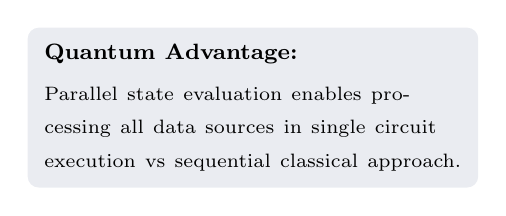
\begin{tikzpicture}
            \node[rounded corners=4pt, fill=primaryblue!10, inner sep=6pt, text width=5.3cm] {
                \footnotesize\textbf{Quantum Advantage:}\\[0.1cm]
                \scriptsize Parallel state evaluation enables processing all data sources in single circuit execution vs sequential classical approach.
            };
        \end{tikzpicture}
    \end{column}
\end{columns}
\end{frame}

% ============================================
% SLIDE 8: QUANTUM ENTANGLEMENT
% ============================================
\begin{frame}{Methodology: Quantum Entanglement Correlation Analysis}

\begin{columns}[T]
    \begin{column}{0.50\textwidth}
        \textbf{\color{primaryblue}\small Purpose}
        \vspace{0.05cm}

        \footnotesize
        Detect correlations between environmental parameters efficiently

        \vspace{0.15cm}
        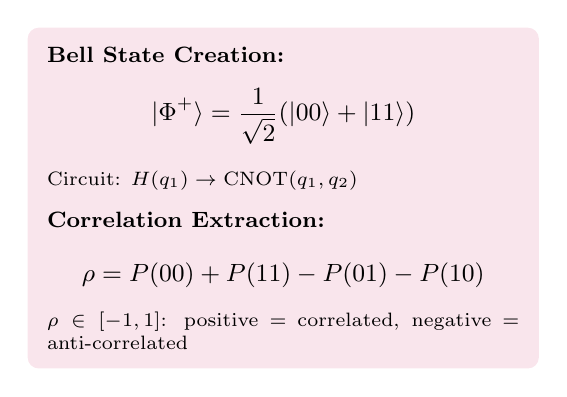
\begin{tikzpicture}
            \node[rounded corners=4pt, fill=purple!10, inner sep=7pt] {
                \begin{minipage}{6cm}
                    \footnotesize\textbf{Bell State Creation:}
                    \small
                    $$|\Phi^+\rangle = \frac{1}{\sqrt{2}}(|00\rangle + |11\rangle)$$

                    \scriptsize Circuit: $H(q_1) \rightarrow \text{CNOT}(q_1, q_2)$

                    \vspace{0.15cm}
                    \footnotesize\textbf{Correlation Extraction:}
                    \small
                    $$\rho = P(00) + P(11) - P(01) - P(10)$$

                    \scriptsize $\rho \in [-1, 1]$: positive = correlated, negative = anti-correlated
                \end{minipage}
            };
        \end{tikzpicture}

        \vspace{0.15cm}

        \textbf{\color{primaryblue}\footnotesize Discovered Correlations}
        \vspace{0.1cm}

        \scriptsize
        \renewcommand{\arraystretch}{1.15}
        \begin{tabular}{p{3.2cm}c}
            \rowcolor{primaryblue!10}
            \textbf{Parameter Pair} & \textbf{$\rho$} \\
            PM$_{2.5}$ -- PM$_{10}$ & 0.92 \\
            \rowcolor{softgray}
            Temperature -- Ozone & 0.78 \\
            Wind Speed -- Pollutants & $-0.81$ \\
        \end{tabular}
    \end{column}

    \begin{column}{0.47\textwidth}
        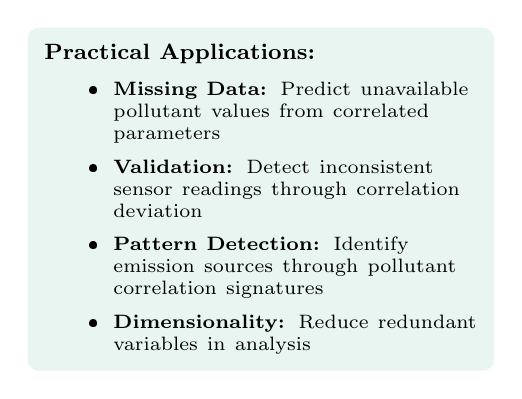
\begin{tikzpicture}
            \node[rounded corners=4pt, fill=mintgreen!40, inner sep=6pt, text width=5.5cm] {
                \footnotesize\textbf{Practical Applications:}\\[0.1cm]
                \scriptsize
                \begin{itemize}\setlength{\itemsep}{2pt}
                    \item \textbf{Missing Data:} Predict unavailable pollutant values from correlated parameters
                    \item \textbf{Validation:} Detect inconsistent sensor readings through correlation deviation
                    \item \textbf{Pattern Detection:} Identify emission sources through pollutant correlation signatures
                    \item \textbf{Dimensionality:} Reduce redundant variables in analysis
                \end{itemize}
            };
        \end{tikzpicture}

        \vspace{0.15cm}

        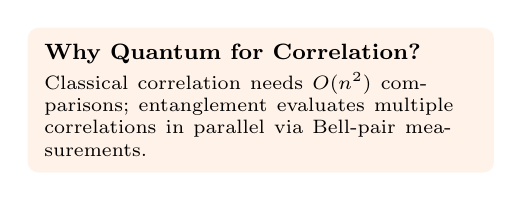
\begin{tikzpicture}
            \node[rounded corners=4pt, fill=warmpeach!35, inner sep=6pt, text width=5.5cm] {
                \footnotesize\textbf{Why Quantum for Correlation?}\\[0.1cm]
                \scriptsize Classical correlation needs $O(n^2)$ comparisons; entanglement evaluates multiple correlations in parallel via Bell-pair measurements.

            };
        \end{tikzpicture}

        \vspace{0.15cm}

        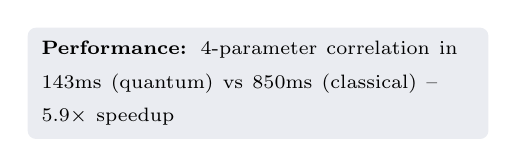
\begin{tikzpicture}
            \node[rounded corners=3pt, fill=primaryblue!10, inner sep=5pt, text width=5.5cm] {
                \scriptsize\textbf{Performance:} 4-parameter correlation in 143ms (quantum) vs 850ms (classical) -- 5.9$\times$ speedup
            };
        \end{tikzpicture}
    \end{column}
\end{columns}
\end{frame}

% ============================================
% SLIDE 9: RESULTS - PERFORMANCE
% ============================================
\begin{frame}{Results: Processing Performance}
\begin{columns}[T]
    \begin{column}{0.50\textwidth}
        \textbf{\color{primaryblue}\small Quantum vs Classical Comparison}
        \vspace{0.1cm}

        \scriptsize
        \renewcommand{\arraystretch}{1.2}
        \begin{tabular}{p{2.2cm}ccc}
            \rowcolor{primaryblue!15}
            \textbf{Task} & \textbf{Classical} & \textbf{Quantum} & \textbf{Speedup} \\
            4-source fusion & 600ms & 87ms & 6.9$\times$ \\
            \rowcolor{softgray}
            8-source fusion & 1200ms & 124ms & 9.7$\times$ \\
            Correlation (4p) & 850ms & 143ms & 5.9$\times$ \\
            \rowcolor{softgray}
            Optimal selection & 640ms & 95ms & 6.7$\times$ \\
        \end{tabular}

        \vspace{0.2cm}

        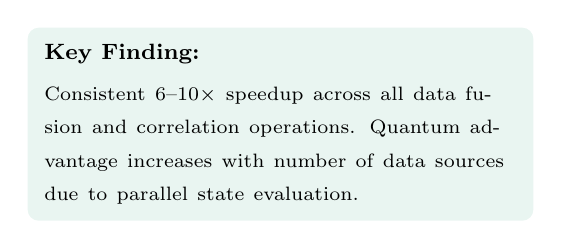
\begin{tikzpicture}
            \node[rounded corners=4pt, fill=mintgreen!40, inner sep=6pt, text width=6cm] {
                \footnotesize\textbf{Key Finding:}\\[0.1cm]
                \scriptsize Consistent 6--10$\times$ speedup across all data fusion and correlation operations. Quantum advantage increases with number of data sources due to parallel state evaluation.
            };
        \end{tikzpicture}

        \vspace{0.15cm}

        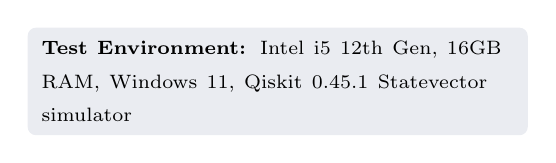
\begin{tikzpicture}
            \node[rounded corners=3pt, fill=primaryblue!10, inner sep=5pt, text width=6cm] {
                \scriptsize\textbf{Test Environment:} Intel i5 12th Gen, 16GB RAM, Windows 11, Qiskit 0.45.1 Statevector simulator
            };
        \end{tikzpicture}
    \end{column}

    \begin{column}{0.47\textwidth}
        \textbf{\color{primaryblue}\small System Response Times}
        \vspace{0.1cm}

        \scriptsize
        \renewcommand{\arraystretch}{1.2}
        \begin{tabular}{p{2.4cm}cc}
            \rowcolor{accentteal!15}
            \textbf{Operation} & \textbf{Target} & \textbf{Achieved} \\
            AQI Calculation & $<$500ms & 287ms \\
            \rowcolor{softgray}
            Layer Rendering & $<$2s & 1.2s \\
            Map Tile Generation & $<$1s & 0.4s \\
            \rowcolor{softgray}
            Location Search & $<$1s & 0.6s \\
            PDF Report (25pg) & $<$30s & 18s \\
            \rowcolor{softgray}
            IDW Grid (100k pts) & $<$5s & 2.4s \\
        \end{tabular}

        \vspace{0.2cm}

        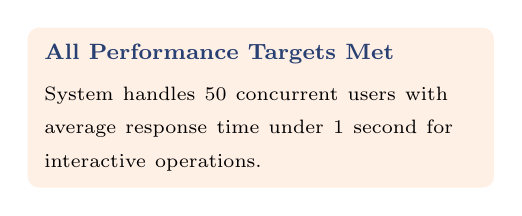
\begin{tikzpicture}
            \node[rounded corners=4pt, fill=warmpeach!40, inner sep=6pt, text width=5.5cm] {
                \footnotesize\textbf{\color{primaryblue}All Performance Targets Met}\\[0.1cm]
                \scriptsize System handles 50 concurrent users with average response time under 1 second for interactive operations.
            };
        \end{tikzpicture}

        \vspace{0.15cm}

        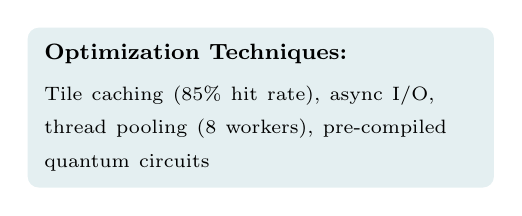
\begin{tikzpicture}
            \node[rounded corners=4pt, fill=accentteal!15, inner sep=6pt, text width=5.5cm] {
                \footnotesize\textbf{Optimization Techniques:}\\[0.1cm]
                \scriptsize Tile caching (85\% hit rate), async I/O, thread pooling (8 workers), pre-compiled quantum circuits
            };
        \end{tikzpicture}
    \end{column}
\end{columns}
\end{frame}

% ============================================
% SLIDE 10: RESULTS - DELIVERABLES
% ============================================
\begin{frame}{Results: Platform Deliverables}
\begin{columns}[T]
    \begin{column}{0.48\textwidth}
        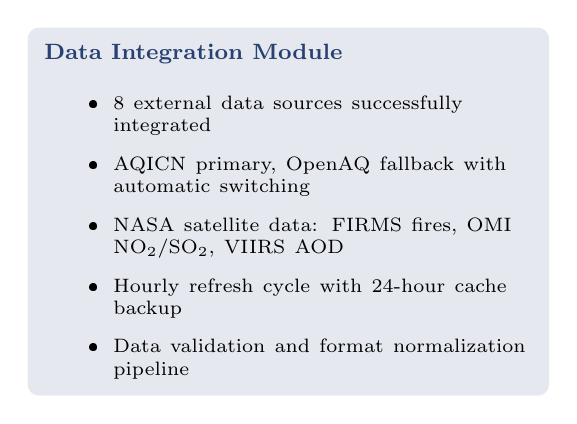
\begin{tikzpicture}
            \node[rounded corners=4pt, fill=primaryblue!12, inner sep=6pt, text width=6.2cm] {
                \textbf{\color{primaryblue}\footnotesize Data Integration Module}\\[0.1cm]
                \scriptsize
                \begin{itemize}\setlength{\itemsep}{2pt}
                    \item 8 external data sources successfully integrated
                    \item AQICN primary, OpenAQ fallback with automatic switching
                    \item NASA satellite data: FIRMS fires, OMI NO$_2$/SO$_2$, VIIRS AOD
                    \item Hourly refresh cycle with 24-hour cache backup
                    \item Data validation and format normalization pipeline
                \end{itemize}
            };
        \end{tikzpicture}

        \vspace{0.12cm}

        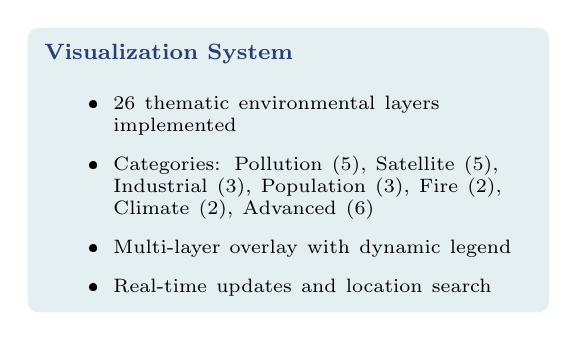
\begin{tikzpicture}
            \node[rounded corners=4pt, fill=accentteal!15, inner sep=6pt, text width=6.2cm] {
                \textbf{\color{primaryblue}\footnotesize Visualization System}\\[0.1cm]
                \scriptsize
                \begin{itemize}\setlength{\itemsep}{2pt}
                    \item 26 thematic environmental layers implemented
                    \item Categories: Pollution (5), Satellite (5), Industrial (3), Population (3), Fire (2), Climate (2), Advanced (6)
                    \item Multi-layer overlay with dynamic legend
                    \item Real-time updates and location search
                \end{itemize}
            };
        \end{tikzpicture}
    \end{column}

    \begin{column}{0.48\textwidth}
        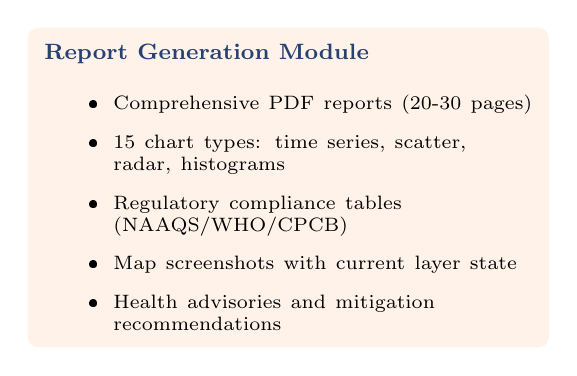
\begin{tikzpicture}
            \node[rounded corners=4pt, fill=warmpeach!35, inner sep=6pt, text width=6.2cm] {
                \textbf{\color{primaryblue}\footnotesize Report Generation Module}\\[0.1cm]
                \scriptsize
                \begin{itemize}\setlength{\itemsep}{2pt}
                    \item Comprehensive PDF reports (20-30 pages)
                    \item 15 chart types: time series, scatter, radar, histograms
                    \item Regulatory compliance tables (NAAQS/WHO/CPCB)
                    \item Map screenshots with current layer state
                    \item Health advisories and mitigation recommendations
                \end{itemize}
            };
        \end{tikzpicture}

        \vspace{0.12cm}

        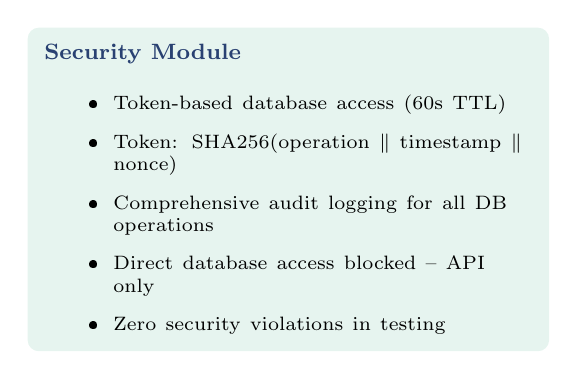
\begin{tikzpicture}
            \node[rounded corners=4pt, fill=mintgreen!45, inner sep=6pt, text width=6.2cm] {
                \textbf{\color{primaryblue}\footnotesize Security Module}\\[0.1cm]
                \scriptsize
                \begin{itemize}\setlength{\itemsep}{2pt}
                    \item Token-based database access (60s TTL)
                    \item Token: SHA256(operation $\|$ timestamp $\|$ nonce)
                    \item Comprehensive audit logging for all DB operations
                    \item Direct database access blocked -- API only
                    \item Zero security violations in testing
                \end{itemize}
            };
        \end{tikzpicture}
    \end{column}
\end{columns}
\end{frame}

% ============================================
% SLIDE 11: PROJECT STATUS
% ============================================
\begin{frame}{Project Status}
\begin{center}
    
\begin{tikzpicture}
        \node[rounded corners=5pt, fill=primaryblue!15, inner sep=7pt] {
            \normalsize\textbf{\color{primaryblue}Overall Project Completion: 95.7\%}
        };
    \end{tikzpicture}
\end{center}

\vspace{0.1cm}

\begin{columns}[T]
    \begin{column}{0.58\textwidth}
        \scriptsize
        \renewcommand{\arraystretch}{1.08}
        \begin{tabular}{p{2.6cm}cp{4.2cm}}
            \rowcolor{primaryblue!12}
            \textbf{Module} & \textbf{Status} & \textbf{Notes} \\
            Backend Core & 100\% & All API endpoints operational \\
            \rowcolor{softgray}
            Data Integration & 95\% & 8 sources integrated; edge cases pending \\
            Core Algorithms & 100\% & Validated against CPCB reference \\
            \rowcolor{softgray}
            Quantum Module & 90\% & Functional; documentation pending \\
            Security Layer & 100\% & Token auth and audit logging active \\
            \rowcolor{softgray}
            Frontend Core & 100\% & Cross-browser tested \\
            Layer Components & 92\% & 24/26 layers polished \\
            \rowcolor{softgray}
            PDF Generation & 95\% & Chart optimization pending \\
            UI/UX Design & 100\% & Desktop and mobile complete \\
            \rowcolor{softgray}
            Testing & 85\% & Integration tests complete \\
        \end{tabular}
    \end{column}

    \begin{column}{0.40\textwidth}
        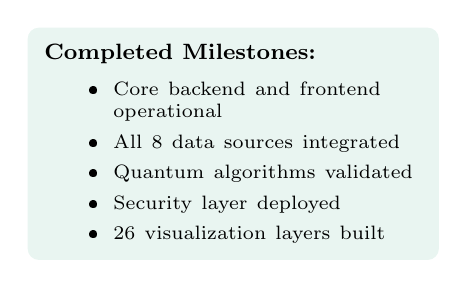
\begin{tikzpicture}
            \node[rounded corners=4pt, fill=mintgreen!40, inner sep=6pt, text width=4.8cm] {
                \footnotesize\textbf{Completed Milestones:}\\[0.1cm]
                \scriptsize
                \begin{itemize}\setlength{\itemsep}{1pt}
                    \item Core backend and frontend operational
                    \item All 8 data sources integrated
                    \item Quantum algorithms validated
                    \item Security layer deployed
                    \item 26 visualization layers built
                \end{itemize}
            };
        \end{tikzpicture}

        \vspace{0.12cm}

        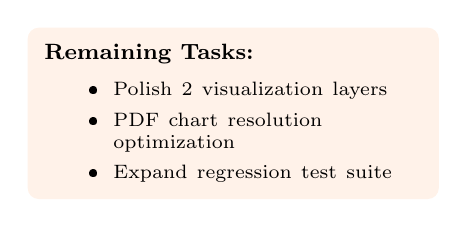
\begin{tikzpicture}
            \node[rounded corners=4pt, fill=warmpeach!35, inner sep=6pt, text width=4.8cm] {
                \footnotesize\textbf{Remaining Tasks:}\\[0.1cm]
                \scriptsize
                \begin{itemize}\setlength{\itemsep}{1pt}
                    \item Polish 2 visualization layers
                    \item PDF chart resolution optimization
                    \item Expand regression test suite
                \end{itemize}
            };
        \end{tikzpicture}

        \vspace{0.12cm}

        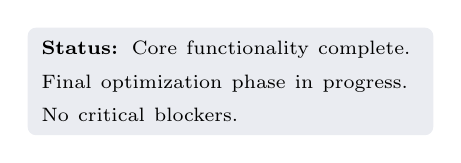
\begin{tikzpicture}
            \node[rounded corners=3pt, fill=primaryblue!10, inner sep=5pt, text width=4.8cm] {
                \scriptsize\textbf{Status:} Core functionality complete. Final optimization phase in progress. No critical blockers.
            };
        \end{tikzpicture}
    \end{column}
\end{columns}
\end{frame}

% ============================================
% SLIDE 12: FUTURE DIRECTIONS
% ============================================
\begin{frame}{Future Directions}
\begin{columns}[T]
    \begin{column}{0.48\textwidth}
        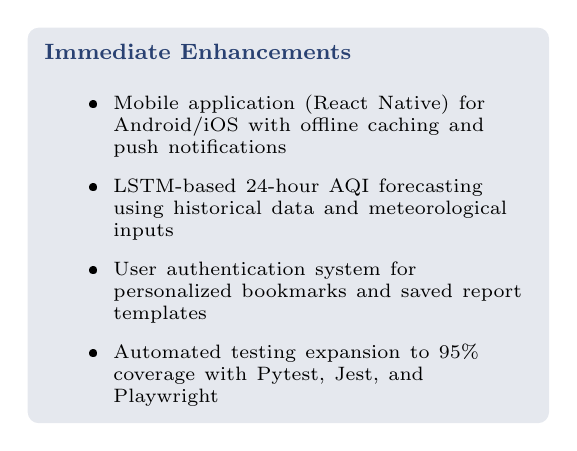
\begin{tikzpicture}
            \node[rounded corners=4pt, fill=primaryblue!12, inner sep=6pt, text width=6.2cm] {
                \textbf{\color{primaryblue}\footnotesize Immediate Enhancements}\\[0.1cm]
                \scriptsize
                \begin{itemize}\setlength{\itemsep}{2pt}
                    \item Mobile application (React Native) for Android/iOS with offline caching and push notifications
                    \item LSTM-based 24-hour AQI forecasting using historical data and meteorological inputs
                    \item User authentication system for personalized bookmarks and saved report templates
                    \item Automated testing expansion to 95\% coverage with Pytest, Jest, and Playwright
                \end{itemize}
            };
        \end{tikzpicture}

        \vspace{0.12cm}

        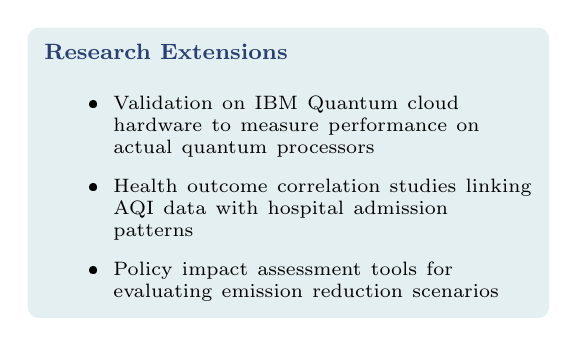
\begin{tikzpicture}
            \node[rounded corners=4pt, fill=accentteal!15, inner sep=6pt, text width=6.2cm] {
                \textbf{\color{primaryblue}\footnotesize Research Extensions}\\[0.1cm]
                \scriptsize
                \begin{itemize}\setlength{\itemsep}{2pt}
                    \item Validation on IBM Quantum cloud hardware to measure performance on actual quantum processors
                    \item Health outcome correlation studies linking AQI data with hospital admission patterns
                    \item Policy impact assessment tools for evaluating emission reduction scenarios
                \end{itemize}
            };
        \end{tikzpicture}
    \end{column}

    \begin{column}{0.48\textwidth}
        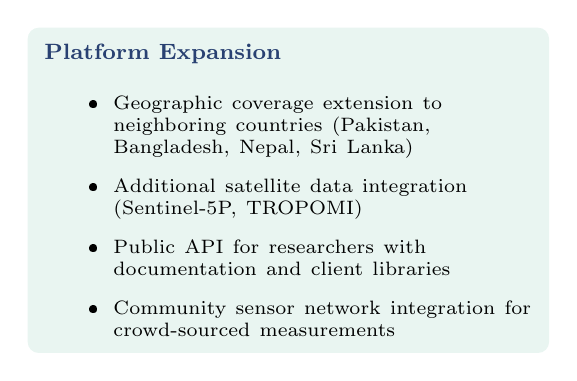
\begin{tikzpicture}
            \node[rounded corners=4pt, fill=mintgreen!40, inner sep=6pt, text width=6.2cm] {
                \textbf{\color{primaryblue}\footnotesize Platform Expansion}\\[0.1cm]
                \scriptsize
                \begin{itemize}\setlength{\itemsep}{2pt}
                    \item Geographic coverage extension to neighboring countries (Pakistan, Bangladesh, Nepal, Sri Lanka)
                    \item Additional satellite data integration (Sentinel-5P, TROPOMI)
                    \item Public API for researchers with documentation and client libraries
                    \item Community sensor network integration for crowd-sourced measurements
                \end{itemize}
            };
        \end{tikzpicture}

        \vspace{0.12cm}

        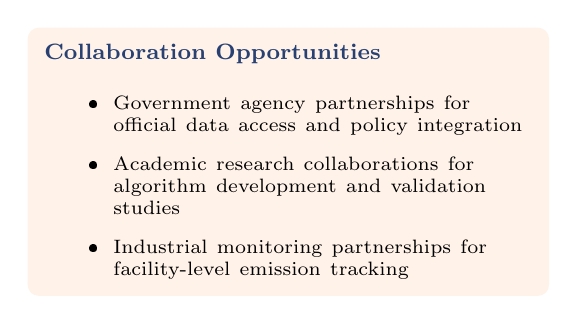
\begin{tikzpicture}
            \node[rounded corners=4pt, fill=warmpeach!35, inner sep=6pt, text width=6.2cm] {
                \textbf{\color{primaryblue}\footnotesize Collaboration Opportunities}\\[0.1cm]
                \scriptsize
                \begin{itemize}\setlength{\itemsep}{2pt}
                    \item Government agency partnerships for official data access and policy integration
                    \item Academic research collaborations for algorithm development and validation studies
                    \item Industrial monitoring partnerships for facility-level emission tracking
                \end{itemize}
            };
        \end{tikzpicture}
    \end{column}
\end{columns}
\end{frame}

% ============================================
% SLIDE 13: CONCLUSION
% ============================================
\begin{frame}[plain]
\begin{tikzpicture}[remember picture,overlay]
    \fill[softcream] (current page.south west) rectangle (current page.north east);
    \fill[primaryblue!12] ([xshift=-1cm]current page.north west)
        .. controls +(4,-0.5) and +(-2,1.5) .. ([xshift=5cm,yshift=-1.2cm]current page.north west)
        -- ([xshift=-1cm,yshift=-1.2cm]current page.north west) -- cycle;
    \fill[accentteal!10] ([xshift=1cm]current page.south east)
        .. controls +(-4,0.5) and +(2,-1.5) .. ([xshift=-5cm,yshift=1.5cm]current page.south east)
        -- ([xshift=1cm,yshift=1.5cm]current page.south east) -- cycle;
\end{tikzpicture}

\vspace{0.3cm}
\begin{center}
    {\Large\bfseries\color{primaryblue} Conclusion}
    
\begin{tikzpicture}
        \fill[accentteal] (-1.2,0) rectangle (1.2,1.5pt);
    \end{tikzpicture}
\end{center}

\vspace{0.1cm}

\begin{center}
\begin{tikzpicture}
    \node[rounded corners=5pt, fill=white, drop shadow={opacity=0.12}, inner sep=10pt, text width=13cm] {
        \small
        \textbf{\color{primaryblue}AetherScan} provides a unified environmental intelligence platform addressing critical gaps in air quality monitoring infrastructure across India.

        \vspace{0.15cm}
        \textbf{\color{primaryblue}Key Technical Contributions:}
        \begin{enumerate}\setlength{\itemsep}{2pt}
            \item \textbf{Data Integration:} Unified pipeline aggregating eight authoritative environmental data sources with automatic failover
            \item \textbf{Quantum Processing:} Demonstrated 6--10$\times$ performance improvement using Qiskit superposition and entanglement algorithms
            \item \textbf{Spatial Analysis:} KD-tree optimized IDW interpolation providing continuous coverage from sparse monitoring networks
            \item \textbf{Visualization:} 26 interactive environmental layers with comprehensive PDF reporting and regulatory compliance assessment
        \end{enumerate}

        \vspace{0.1cm}
        \textbf{\color{primaryblue}Impact:} Enables environmental researchers, government agencies, and citizens to access comprehensive air quality data and analysis tools for informed decision-making.
    };
\end{tikzpicture}
\end{center}

\vspace{0.2cm}

\begin{center}
    {\large\color{primaryblue}\textbf{Thank You}}
\end{center}
\vspace{0.2cm}
\end{frame}

\end{document}
